% !TEX TS-program = pdflatex
% !TEX encoding = UTF-8 Unicode

% This is a simple template for a LaTeX document using the "article" class.
% See "book", "report", "letter" for other types of document.

\documentclass[11pt]{article} % use larger type; default would be 10pt

\usepackage[utf8]{inputenc} % set input encoding (not needed with XeLaTeX)
\usepackage{biblatex} %Imports biblatex package
\addbibresource{Black-Scholes.bib} %Import the bibliography file
\usepackage{graphicx}
\graphicspath{ {./images/} }

%%% Examples of Article customizations
% These packages are optional, depending whether you want the features they provide.
% See the LaTeX Companion or other references for full infofrmation.

%%% PAGE DIMENSIONS
\usepackage{geometry} % to change the page dimensions
\geometry{a4paper} % or letterpaper (US) or a5paper or....
% \geometry{margin=2in} % for example, change the margins to 2 inches all round
% \geometry{landscape} % set up the page for landscape
%   read geometry.pdf for detailed page layout information

\usepackage{graphicx} % support the \includegraphics command and options

% \usepackage[parfill]{parskip} % Activate to begin paragraphs with an empty line rather than an indent

%%% PACKAGES
%\usepackage{hyperef}
\usepackage{booktabs} % for much better looking tables
\usepackage[english]{babel}
\usepackage{amsthm}

\usepackage{amsmath}
\usepackage{array} % for better arrays (eg matrices) in maths
\usepackage{paralist} % very flexible & customisable lists (eg. enumerate/itemize, etc.)
\usepackage{verbatim} % adds environment for commenting out blocks of text & for better verbatim
\usepackage{subfig} % make it possible to include more than one captioned figure/table in a single float
% These packages are all incorporated in the memoir class to one degree or another...

%%% HEADERS & FOOTERS
\usepackage{fancyhdr} % This should be set AFTER setting up the page geometry
\pagestyle{fancy} % options: empty , plain , fancy
\renewcommand{\headrulewidth}{0pt} % customise the layout...
\lhead{}\chead{}\rhead{}
\lfoot{}\cfoot{\thepage}\rfoot{}

%%% SECTION TITLE APPEARANCE
\usepackage{sectsty}
\allsectionsfont{\sffamily\mdseries\upshape} % (See the fntguide.pdf for font help)
% (This matches ConTeXt defaults)

%%% ToC (table of contents) APPEARANCE

\usepackage{amsfonts} 
\usepackage[nottoc,notlof,notlot]{tocbibind} % Put the bibliography in the ToC
\usepackage[titles,subfigure]{tocloft} % Alter the style of the Table of Contents
\renewcommand{\cftsecfont}{\rmfamily\mdseries\upshape}
\renewcommand{\cftsecpagefont}{\rmfamily\mdseries\upshape} % No bold!
%%% END Article customizations

\newtheorem{theorem}{Theorem}[section]
\newtheorem{corollary}{Corollary}[theorem]
\newtheorem{lemma}[theorem]{Lemma}


%%% The "real" document content comes below...

\title{GameStop: A study in the Black-Scholes Formula}
\author{Luke Stanislaus 2009701}
%\date{} % Activate to display a given date or no date (if empty),
         % otherwise the current date is printed 

\begin{document}

\maketitle
\tableofcontents
\begin{abstract}
    This essay is about the Black-Scholes formula, and how it could be 
    used to explain the short squeeze of GameStop in early 2021. We begin 
    with explaining shares, options and short selling, and move on to 
    deriving the Black-Scholes formula, and finally apply it to GameStop.
    \end{abstract}

%\section{Introduction}


\section{What are shares, options, and short selling?}
\subsection{Shares}
As defined in~\cite{shares}, shares are ``units of equity 
ownership in a corporation''. Writing shares can be an effective way to raise 
capital for a firm, as there is no legal mandate to be repaid to 
investors, and they do not need to pay interest. However, common shares usually offer voting 
rights, giving shareholders control over a business. There can be some cases 
of businesses where being private means it can struggle to functions effectively.
For example, SpaceX, owned by Elon Musk, has remained a private company, as 
shareholders can tend to look very closely at short term profits, taking less 
consideringinto the long term of a company, and a space launch company can 
struggle to create consistent income, and in this case a small group of investors 
who are fully onboard with the company vision will allow the company to lose 
money in the short term in order to gain longer term profits. This was also 
the plan with Tesla, as the company struggled to scale up production of its new 
car and had to spend lots of money in research. 
\paragraph{}
The value of 
shares rises and falls with demand - meaning that owning a stock assumes 
the owner a certain level of risk. Many stocks also offer dividends to 
shareholders, which is a proportion of the business's profits paid out 
directly and allows low growth, highly profitable business to offer value 
to shareholders.
\subsection{Options}
Again, as defined in~\cite{options}, ``the term option refers to a 
financial instrument based on the value of the underlying security, 
such as stocks''. An options contract offers the holder the option, 
not the obligation (in contrast to a ``future''), to buy or sell a share 
at a predetermined price. In themselves, they are a form of asset and 
as such have their own valuations and market value. A ``call'' option 
is when the writer of the option promises to sell the stock at a 
predetermined price, (called the ``strike'') at a predetermined time, 
(called the ``exercise date''). This means that if you own a call option and 
the stock price increases above the strike price, the writer will still have 
to honor the strike and so you can ``exercise'' the option 
and immediately sell the stock, where your profit is the difference 
between the strike and current price, less the cost of the option. 
However, if the price goes below the strike, you would be forced 
to let your option expire worthless, since by exercising the option, 
you would pay above the market rate. In this way, the losses are limited 
but the profits are unlimited - you can only lose what you paid for the 
call options but stand to gain an unlimited amount as the stock price 
increases. 
\paragraph{}
On the other hand, if an investor expects a stock to decrease 
in value, they could write a call (also known as a short call). This 
means that if the stock has increase in value and you don't already own 
the security, you are obligated to purchase at the market rate, which 
could take any arbitrary value. Further to this, as the price increases 
over time, the short seller may be ``margin called'' - when to ensure the 
seller can pay, the broker requests that the seller puts more money into 
their account. If the short seller cannot afford this (and the further 
risk it entails), they can close their position - by buying the stocks 
they owe, they are protected from any further increases in price. However, 
by buying the stock off the open market they increase demand for the 
stock, increasing the price further, forcing other short sellers to 
close their positions, driving the price up further. This is what is 
known as a short squeeze. There isn't really a symmetrical ``long 
squeeze'' - the lowest a stock can be valued is zero, so is limited to the 
value of the stocks sold long, hence a short squeeze is a unique phenomenon in 
this respect.
\paragraph{}\label{typesofoption}
There are also two types of options - a ``European'' and ``American'' 
derivative security. An European option can only be exercised at the 
exercise date, while an American option can be exercised at any time up 
to the exercise date. In this essay we shall only consider the simpler 
European option, although the American option is far more common in 
the financial markets. 

\section{Short squeezes and GameStop}
A short squeeze is relatively uncommon occurence in financial markets, but they do 
happen, normally due to substantial short interest in the stock, i.e.,\  a large number 
of the shares sold short, an a small available float - the number of shares 
available to purchase on the market. This means, as the short sellers (traders 
writing call options) are forced to close their positions, they are fighting over 
a small number of stocks, inflating the price to extraordinary values. 
\paragraph{}
An extreme of an extremely artificial short squeeze was Volkswagen in 2008, where 
Porsche began to buy large amounts of Volkswagen stock off the market, as they were looking 
to purchase the business. This 
meant that only 6\% of the stock was available on the market, while 13\% of the stock 
was sold short. Th\begin{figure}[h]
    \centering
    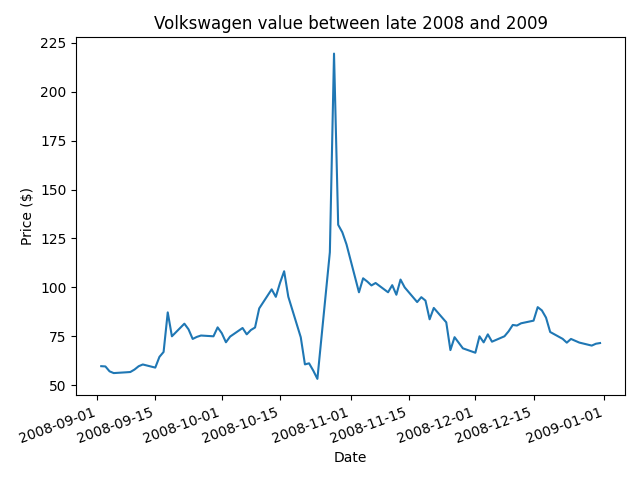
\includegraphics[width=0.55\textwidth]{volkswagenShortSqueeze.png}
    \caption{The stock price of Volkswagen during the short squeeze of 2008}
    \end{figure}is caused a scramble for the final few shares, and as short sellers 
were squeezed out by the high price and were forced to close their position by buying 
more of the stock, the price went higher and higher, and Volkswagen briefly became 
the highest value company in the world, reaching a peak value of around \$1000, up from 
around \$50 just before. The squeeze only ended when Porsche announced 
it would sell around 5\% of its stake in order to make life easier for the hedge 
funds - it is estimated that the squeeze cost short sellers around £30 billion, 
according to~\cite{volkswagen}, with massive profits going over to Porsche, during 
a financial crisis! In total, it is estimated that the short squeeze cost short 
sellers around £30 billion~\cite{volkswagen}. 

\paragraph{}
The case of GameStop is similar - there was an extreme amount of short interest in 
the share, so that at one point more than 100\% of the stock was sold short. With 
\begin{figure}[h]
    \centering
    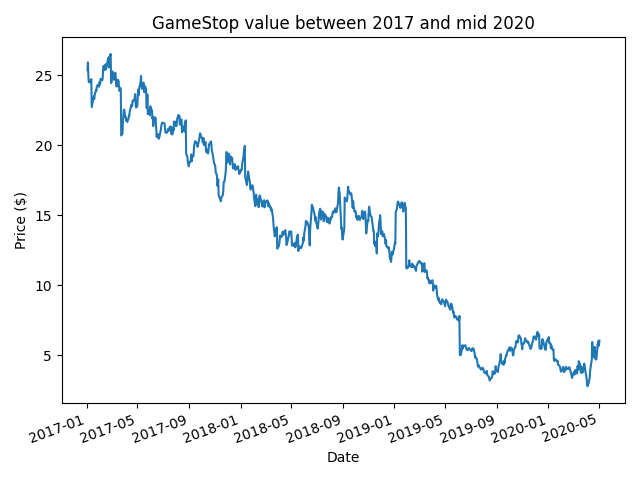
\includegraphics[width=0.55\textwidth]{gameStopPriorValue.png}
    \caption{GameStop daily closing price, data from~\cite{nasdaq} }\label{gamestopprice}
    \end{figure}
    COVID and the death of the high street, a brick-and-mortar store like GameStop was 
considered an extremely safe short sell - and as you can see from~\ref{gamestopprice}  
until mid 2020, the price of GameStop was dropping extremely consistently. As we shall study, 
a low volatility history will mean that short sellers can become highly leveraged against a 
stock, as low stock volatility implies low option volatility - it is very unlikely that 
the short sellers is forced to close their position by their broker due to lack of funds - 
the worst possible outcome for the short seller, as there is a chance that a jump is short 
term the underlying stock drops below its strike price before the option expiry. This  
meant that it had an extremely high short interest, as you can see in~\ref{shortinterest}. 
This was noticed by a message board on the internet, called ``r/wallstreetbets''~\cite{wsb}. 
\begin{figure}[h]
    \centering
    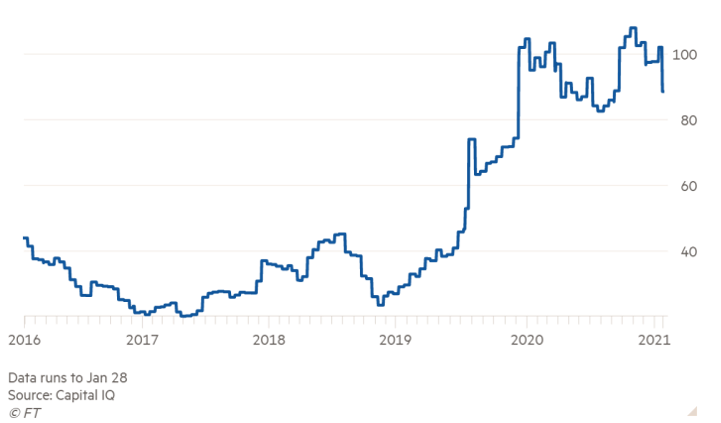
\includegraphics[width=0.55\textwidth]{shortinterest.png}
    \caption{The short interest in GameStop over the past 5 years.}\label{shortinterest}
    \end{figure}
The independent investors saw this as greed from the large hedge funds making billions 
of safe money preying on the demise of a beloved high street store.\  and when Ryan Cohen, 
who had just created the hugely successful 
``Chewy'', the largest online pet retailer, joined GameStop's board as chairman. Investors
on \textit{r/wallstreetbets} saw this as a very positive sign, 
as they envisaged Ryan turning GameStop into Amazon, but for video games. Hence, they 
organised a concerted attempt to create a 
short squeeze in GameStop, hoping to profit from the excessive greed of the hedge funds. They 
began purchasing the stock, both increasing the price and reducing the available float, 
so that as short sellers attempted to close their positions due to rising prices, they 
found themselves fighting over a smaller and smaller number of shares, like the 
Volkswagen case. This caused a significant short squeeze in the price, profiting the 
internet investors who had bought in early on, as seen in~\ref{shortsqueeze}. In fact, I myself 
was a regular visitor to these internet boards, and in early 2020 I myself ended up investing 
10 stocks back when it was worth just \$40 - the period of massive growth afterwards was an 
extremely exciting time for me, however I wasn't able to time the absolute peak!
\begin{figure}[h]
    \centering
    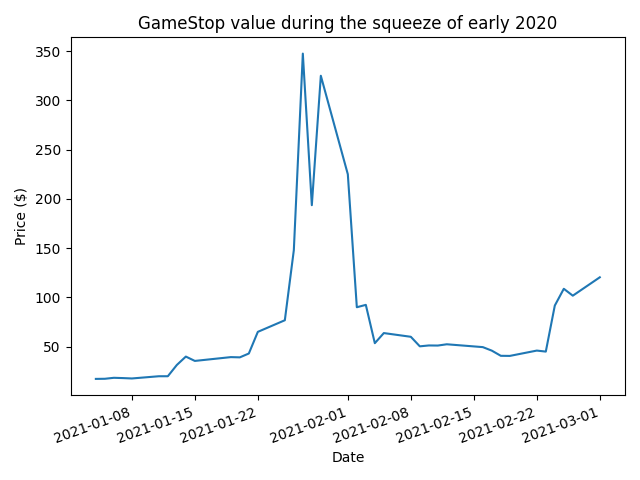
\includegraphics[width=0.55\textwidth]{gameStopSqueezeValue.png}
    \caption{The stock price of GameStop during the squeeze.}\label{shortsqueeze}
    \end{figure}
However, the squeeze was short lived - as the stock increased tenfold, independent 
investors began to cash out on their profits and sell their stock, the pressure 
on the short sellers became reduced and they were able to exit their positions. 
This contrasts with the Volkswagen case, where the shares were all owned by one 
party, who completely refused to sell its shares, pushing the share price much higher. 
\paragraph{}
Meanwhile the messageboards were desperately sharing the message of ``diamond hands'', 
the concept that shareholders should hold onto their stocks, minimizing the available 
float and exacerbating the squeeze. Due to the sheer number of shares sold short on 
the market, it meant that it took much longer for the shorts to unwind their positions 
and so the squeeze lasted a significant amount of the - even now GameStop is worth 
around \$130, far above the low in~\ref{gamestopprice}, which also implies that 
as well as being short squeeze, the share price was more generally undervaluing GameStop.
As particular hedge fund the message boad was targetting was ``Melvin Capital''. This 
fund had a massive short against the GameStop shares, over 2021 ended up losing more 
than \$7 billion. In total it is estimated that short sellers lost around \$20 billion 
over the month of January 2021 to GameStop.

\section{Asset dynamics}\label{assetdyamics}
In our attempt to study the Black-Scholes equation, set out our underlying variables 
and the different variables we need to find in order to study a stock and its options.

\subsection{A risk-free asset}
First we shall define a risk-free asset, which we shall need to define in order to 
calculate the cost of value of an option at time $t$. This is because we can't do 
as described in~\ref{typesofoption}, where we could simply buy another option from the 
market. Since this is what we are trying to calculate, this would make no sense! Therefore, 
The process of finding the risk-free value of an option is detailed in~\ref{riskfreevalue} 
and shall be required in the derivation of the Black-Scholes Model's boundary conditions.
A risk-free asset, as defined in the Black-Scholes Model~\cite{blackscholes} can be thought
of as a money-market account with zero risk, for example a bank account with an interest 
rate. It is described by the deterministic function 
\begin{equation} \label{riskfree}
    dA(t) = rA(t)\mathrm{d}t 
\end{equation}
Where in~\eqref{riskfree}, $r$ represents the risk-free rate and $A$ the value of the 
asset. We typically let $r>0$ and $A(0) = 1$ for convenience. This can be rewritten as 
the ordinary differential equation $A'(t) = rA(t)$, which has the unique solution 
\begin{equation} \label{riskfree solution}
    A(t) =e^{rt}
\end{equation}
\subsection{Ito processes}
Given a Brownian Motion $W(t)$ with filtration $(\mathcal{F}_t, t \geq 0 )$
According to~\cite{itoprocess}, an Ito process is the stochastic (random) 
process $X = \{X_t, t \geq 0\}$ which solves 
\begin{equation} \label{randomprocess}
X_t = X_0 + \int_{0}^{t} a(X_s, s)\mathrm{d}s + 
\int_{0}^{t} b(X_s, s) \mathrm{d}W_s
\end{equation}

Here $a,b$ are stochastic 
processes defined for $\{a(X_t, t) : t\geq0\} $ and $\{b(X_t, t) : t\geq0\}$ which are 
continuous in $t$ and adapted to (can be measured at) our filtration $\mathcal{F}_t$ 
time $t$ and 
both satisfy $c$ in 
\[\int_{0}^{\infty} c(X_s, s) \mathrm{d}s \leq \infty\]
Then we call $a$ the drift of the variable, and $b$ is the diffusion, 
or more precisely in a financial context, volatility.~\eqref{randomprocess} is commonly 
written as 
\begin{equation}
    X_t = a(X_t, t)\mathrm{d}t + b(X_t, t)\mathrm{d}W_t
\end{equation}
or even 
\begin{equation} \label{itoprocess}
    X_t = a_t\mathrm{d}t + b_t\mathrm{d}W_t
\end{equation}
This converges at some time $T$ to Brownian motion with instantaneous drift $a_T$ and
variance $b_T^2$. We let $dW$ be normally distributed with mean zero and variance 
$\mathrm{d}t$. This can also be written discretely as 
\begin{equation}
    \mathrm{d}X_t = a_t\mathrm{d}t + b_t \sqrt{\mathrm{d}t}\xi
\end{equation}
where
\begin{equation}
    \xi \sim \mathcal{N}(1,\,0)
\end{equation}

\subsection{A risky asset}

A risky asset, as defined in The Black-Scholes Model~\cite{blackscholes}, 
can be thought of as a stock, is represented as the Ito process

\begin{equation} \label{riskyasset}
    \mathrm{d}S(t) = \mu S(t)\mathrm{d}t + \sigma S(t) \mathrm{d}W(t)
\end{equation}

with $S(0)$ a given starting price of the stock, $\mu \in \mathbb{R}$ 
is again the drift and $\sigma > 0$ is the volatility of the stock 
price $S$. Using Theorem~\eqref{isosexistence} we can prove existence and uniqueness of 
the solution to  
~\eqref{riskyasset}:

First we rewrite~\eqref{riskyasset} in integral form:
\begin{equation}\label{riskyint}
    S(t) = S(0) + \mu\int_0^t \! S(u) \, \mathrm{d}u + \sigma\int_0^t \! S(u) \, 
    \mathrm{d}W(u).
\end{equation}

Then we rewrite our coefficients in the form of~\eqref{randomprocess}: 

\begin{align}
    \mu S(t) = a(t,S(t)), && a(t,x) = \mu x \\
    \sigma S(t) = b(t,S(t), && b(t,x) = \sigma x
\end{align}

then we check Lipschitz continuity:

\begin{align}
    |a(t,x) - a(t,y)| &= |\mu(x-y)| \leq |\mu||x-y|, \\
    |b(t,x) - b(t,y)| &= |\sigma(x-y)| \leq \sigma|x-y| &&\text{Since $\sigma > 0$.}
\end{align}

We then have that the unique solution to~\eqref{riskyasset} is of the form 
\begin{equation}\label{riskysolution}
    S(t) = S(0)\exp\{\mu t - \frac{\sigma^2}{2}t + \sigma W(t)\}.
\end{equation}
This can be easily substituted into~\eqref{riskyint} show that this solves~\eqref{riskyasset}.

\subsection{Considering the model parameters}

Now we have derived this risky asset, of which an option will be a derivative, 
we need to ensure that the parameters we find are as accurate as possible. To 
go about this, we can consider $\mathbb{E}(S(t))$:

\begin{align}
    \mathbb{E}(S(t))  = &&S(t)\mathbb{E}(\exp\{\mu - \frac{1}{2}\sigma t + \sigma W(t)\})\\
     \label{variance}= 
     && S(0)\exp\{\mu t - \frac{1}{2}\sigma^2 t\}\mathbb{E}(\exp\{\sigma W(t)\} \\
    \label{result} = && S(0)\exp\{\mu t\}).
\end{align}

Where at~\eqref{variance} we use the fact that 

\begin{equation*}
    \mathbb{E}(\exp\{X\}) = \exp\{\frac{1}{2}Var(X)\}
\end{equation*}

~\eqref{result} then shows that if $\mu = 0$ we know that the expectation of $S(t)$ is 
constant in time - it is not ``drifting'' in any direction, which justifies the 
name of $\mu$ as drift. We can then rearrange for $\mu$:

\begin{equation} \label{mu}
    \mu = \frac{1}{t}\ln{\frac{\mathbb{E}(S(t))}{S(0)}}
\end{equation}

which is the logarithmic return of the expected price.
The variance of the return is 
\begin{align}
    Var(\mu t - \frac{\sigma^2}{2}t + \sigma W(t)) = && Var(\sigma W(t)) \\
    = && \sigma^2t  && \text{since $Var(W(t)) = t$}
\end{align}
as defined in~\cite{blackscholes}. Clearly, we want to try to calculate $\mu$ and 
$\sigma$ to apply to our model.~\eqref{mu} could suggest taking past values of the 
stock value and taking an average to find a value of $\mu$, but according statistical 
theory the accuracy of this is poor - past performance of a stock doesn't imply future 
performance.
We can however much more effectively estimate the volatility. This is found by taking 
the logarithm 
of~\eqref{riskysolution}

\[
    \ln{S(t)} = \ln{S(0)} + (\mu - \frac{1}{2}\sigma^2)t + \sigma W(t)
\]

which we notice is an Ito process with the constant characteristics 
$a(t) = (\mu - \frac{1}{2}\sigma^2)$
 and $b(t) = \sigma$. By~\cite{quadtraticvariation}, we have that for an Ito process
 \begin{equation}
     {(\mathrm{d}S(t))}^2 = b^2(t) \mathrm{d}t
 \end{equation}
 If we then partition $[0,t]$ given by $0 = t_1 < \cdots < t_n = t$ with small mesh max 
 width $[t_{k+1} - t_k]$, we have 
 \begin{equation}
     {(\ln{S(t_{k+1}) - \ln{S(t_k)}})}^2 \approx \sigma^2 \mathrm{d}t
 \end{equation}
then 
\begin{align}
    \sum_k {(\ln{S(t_{k+1}) - \ln{S(t_k)}})}^2 \approx \sigma^2 t\\
    \implies
    \sigma = \sqrt{\frac{1}{2}\sum_k {(\ln{\frac{S(t_{k+1})}{S(t_k)}})}^2}
    \label{volatilityapprox}
\end{align}
which is a good estimate of the volatility coefficient, and is described as the 
``sample volatility''. We shall get concrete data from GameStop and use this formula 
to find our value of volatility later on in this essay.

\section{The Black-Scholes Model}
Starting from the model derived and fully defined in~\ref{blackScholesAppendix}, we may consider final and boundary 
conditions of a European Call, as defined in~\ref{typesofoption}. We define this as 
$C(t,z)$, with exercise price $K$ and expiry date $T$ from above. Now for the final 
condition $t=T$ we appeal to the definition of a call as in~\eqref{initialvalue}:
\begin{equation}
    C(T, z) = \max{(z-K, 0)}
\end{equation}

Now for our boundary conditions again we consider $u$ for $z=0$ and $z \to \infty$. Similarly 
to~\eqref{boundarycondition} we have 
\begin{align}
    C(t, 0) = 0 &&\text{for } t \in (0,T)
\end{align}
Then for $z \to \infty$, again we can ignore out max. However, in this case, we must 
purchase the stock and hold on to it until the exercise date, as we have a 
European option. This money spent on the stock could otherwise be put in a 
money market account, so the profit from exercising the option must account for this.
From~\eqref{riskfree solution}, we get that 
\begin{align}
    C(t,z) = z - Ke^{-r(T-t)} &&\text{as } z \to \infty
\end{align}
We then finally get the following, the Black-Scholes European Call option IBVP:

\begin{align}
    u_t(t,z) +\frac{1}{2}\sigma^2z^2u_{zz}(t,z) + rzu_z(t,z) - ru(t,z) = 0 &&
    \text{for $(t,z) \in (0,T) \times \mathbb{R}_+ $}\\
    \text{with initial condition: } &&
     u(0,z) = \max{(z-K, 0)} \text{, } z \in \mathbb{R}_+ \\
    \text{and boundary conditions: } && 
    u(t, 0) = 0 \text{,  $u(t,z) = z - Ke^{-r(T-t)}$}\\
    \text{as $z \to \infty $,  $t \in [0,T]$}
\end{align}

\section{Modelling GameStop}
We begin by using~\eqref{volatilityapprox} a calculate a value of $\sigma$. Using data from
~\cite{nyse} between 2018 - 2020, I solve $\sigma = 1.0073\dots$. We also set 
$r=1.004$, approximately the average bank rate between 2018 - 2020.
\begin{figure}[h] 
    \centering
    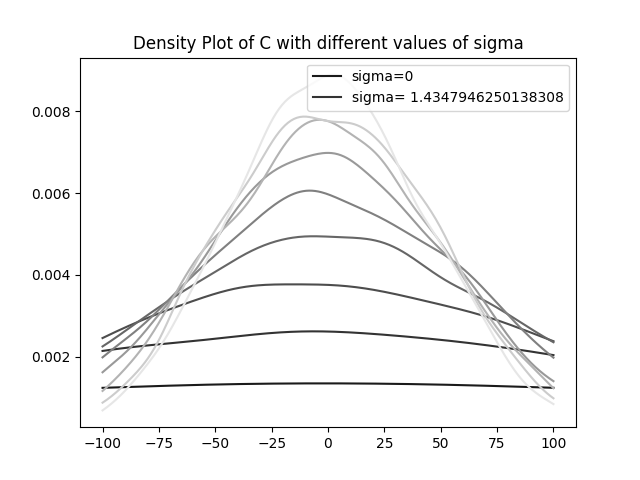
\includegraphics[width=0.5\textwidth]{sigmavalue.png} 
    \caption[]{}\label{sigmavalue}
\end{figure}
~\eqref{sigmavalue} shows how returns from options are far more consistent and safer with a low volatility
stock like in the GameStop case. This relation between volatility in stock compared to 
volatility in option value explains how a short squeeze can be forced to occur - increased 
volatility, not even an increase in the price of the stock, can cause short sellers to be 
margin called, as the broker solves the Black-Scholes PDE and notices the volatility has 
increased substantially. This means that the short seller may be margin called due to 
the increased risk in the option, and may simply decide to close their position, and even though 
stock price may have gone down, the short seller has to buy a stock, pushing the price upwards. 
This explains how only a small number of people can force a short squeeze.
In the above case we have used the solution from~\cite{wikipedia}, 
 so the upper bound to sigma is $x>0$ so:
\begin{align}
    x =&& \ln{\frac{z}{K}} + (r - \frac{1}{2} \sigma^2)\tau > 0 && 
    \text{with $\tau$, $x$ as defined in~\cite{wikipedia}} \\
    \implies |\sigma| <&& \sqrt{\frac{2}{\tau} \ln{\frac{z}{K} + 2r}} && = 1.44\dots
\end{align}
Modifying values of K, the strike price, we see in~\eqref{kvalue} the increased risk 
of buying options with a more expensive strike price, which makes sense - if 
the strike of an option is near the current price, it is more likely that 
the stock drops below this and so expires worthless.
\begin{figure}[h] 
    \centering
    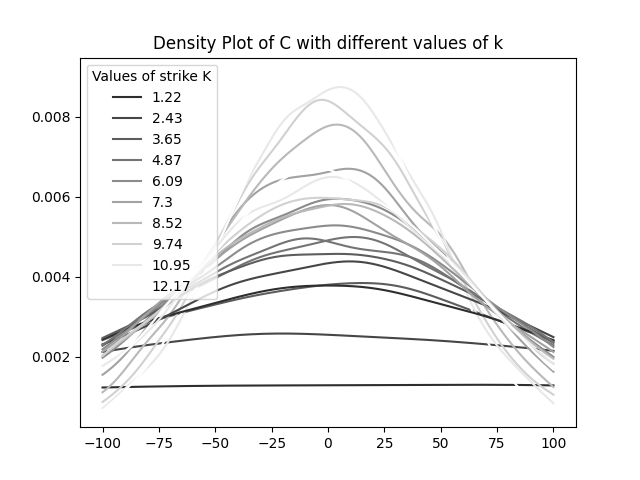
\includegraphics[width=0.5\textwidth]{kvalue.png} 
    \caption[]{}\label{kvalue}
\end{figure}
Again here we have a mathematical limit on the value of k:
\begin{align}
    \ln{\frac{z}{K}} + (r - \frac{1}{2} \sigma^2)\tau > 0 \\
    \implies |k| < ze^{\frac{1}{2}\sigma^2 - r} = 12.17\dots
\end{align}
We finish with an analysis for different values of $\tau$, where we notice that 
the time to expiry has no effect on the distribution of $u$, the value of the 
option.
\begin{figure}[h] 
    \centering
    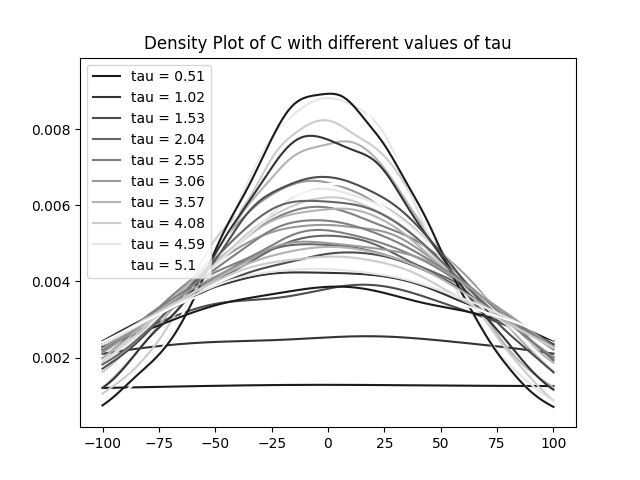
\includegraphics[width=0.5\textwidth]{tauvalue.png} 
    \caption[]{}\label{tauvalue}
\end{figure}
\begin{align}
    \ln{\frac{z}{K}} + (r - \frac{1}{2} \sigma^2)\tau > 0 \\
    \implies |\tau| > \frac{\ln{\frac{K}{z}}}{r - \frac{1}{2}\sigma^2} 
    = -0.05\dots&& \text{although note that time is 
    defined to be non-negative.}
\end{align}
\section{Conclusion}
In conclusion, it is apparent that GameStop was an extremely safe investment 
for these hedge funds - with low volatility and in slow decline, these hedge 
funds could gain millions in low-risk money of the period of many years, which 
is how it ended up gaining such a massive short interest which allowed the 
squeeze to occur so easily. However, this is a perfect example of where 
the Black-Scholes formula becomes extremely ineffective - when there is a 
sudden change in volatility, the Black-Scholes will become a less effective 
model as it essentially expects a stock to perform similarly as in the past, 
so if there is a high volatility (induced, for example, by people on the 
internet) alongside high short interest, due to the way the markets are 
set up billions of dollars can change hands in a very short amount of time!

\printbibliography%Prints bibliography

\appendix

\section{Risk-free value of an option}\label{riskfreevalue}
A key fact to note is that even with a 
European option, all parties involved can close their positions at any time. 
\subsection*{Option holders}
A call options holder has the option to either have the option worth nothing, i.e., 
losing the premium paid, or could lock in the value of the option at time $t$ as 
equal to difference between the strike price and the market price. At time $t$ the 
investor can decide to lock in their profits risk-free, by taking a loan in stocks 
equal to the size of the option and immediately selling the loaned stock. We then give 
the money back to the person who loaned to us, so we pay the risk-free rate. Then at 
expiry, exercise the option and use these stocks to pay back the loan. Then the value is 
the difference between the current price at time $t$ and the strike $K$ plus the 
interest paid $i$ on the loan of the underlying security 
$z$. Considering a call option we have 
 \[C(z,t) = z - (K + i)\]
 and then we calculate interest using~\eqref{riskfree solution} with negative $r$, so 
 over time period $T-t$ where $T$ is expiry, we have risk-free interest paid equal to 
 $z - ze^{-r(T-t)}$ 
 and putting this together we finish with 
 \[
C(z,t) =\max{(0, z - (K + z - ze^{-r(T-t)}))} = \max{(0, ze^{-r(T-t)} - k)}
 \]

\section{Derivation of Black-Scholes Formula}\label{blackScholesAppendix}
\subsection{Assumptions}

As in~\cite{blackscholes}, before we can begin to derive the Black-Scholes Model, we must 
state some assumptions. Note that since the mathematics applied here quickly approaches a 
very high level, I shall brush over some more specific steps while trying to offer a 
satisfying proof of our equation.
\subsubsection{Existence of replicating strategy}\label{replicatingstrategy}

This assumption says that any option investment can be perfectly replicated by holdings in 
the stock and a money market account directly. A key part of investing is the substantial 
``leverage'' employed in an option, as for a small (as a percentage of the share value) cost 
you can purchase many shares and sell them for a profit, without having to risk 
investing such a large amount of money directly into the stock. Our assumption, however, says 
that a ``replicating strategy'' always exists. More rigorously, we say that there exists a 
pair of processes $(x,y)$ which satisfy 
\begin{equation}
    H(t) = x(t)S(t) + y(t)A(t)
\end{equation}
where $H(t)$ is the option value at time T, an Ito proces.$S(t)$ and $A(t)$ are the risky 
and riskless assets as defined in Asset Dynamics~\ref{assetdyamics}. 
As described in~\cite{blackscholes}, this assumption ``captures the idea that changes in the 
values and holdings of assets are sole drivers of changes of wealth''.

Additionally we assume that the process $H(t)$ is of  the form 
\begin{equation}
    H(t) = u(t, S(t)).
\end{equation}

This deterministic function $u(t,z)$ is not dependant on the history of the stock price. 
It is assumed to have continuous first derivative wrt $x \in [0,T]$ and continuous first 
and second derivatives in $z \in \mathbb{R}$.

\subsubsection{Assumption 2}
There again exists a replicating strategy $(x,y)$ which satisfies 
\begin{equation}\label{replicatingderivative}
    \mathrm{d} H(t) = x(t)\mathrm{d} S(t) + y(t)\mathrm{d} A(t)
\end{equation}
where $H$, $S$, $x$, $y$ and $A$ are as defined in~\eqref{replicatingstrategy}.
\subsubsection{Assumption 3}
There exists a probability Q


Applying~\eqref{itolemma} with $u(t,Z) = f(Z)$ we get   
\begin{align}\label{itoformulasolve}
    \mathrm{d}u(Z)  = u_z(Z)\mu \mathrm{d}t + u_z(Z)\sigma \mathrm{d}W + \frac{1}{2}
    u_{zz}(Z) \sigma^2 \mathrm{d}t&& \text{and} \\
    \mathrm{d}u(t) = u_t &&\text{then} \\
    \mathrm{d}H =\mathrm{d}u = \mathrm{d}u(Z) +\mathrm{d}u(t) =   (u_t + \mu S u_z + \frac{1}{2} 
    \sigma^2 S^2 u_{zz})\mathrm{d}t + +\sigma S u_z \mathrm{d}W
\end{align}
as a stochastic differential.
From~\eqref{replicatingderivative}, we have
\begin{align}
    \mathrm{d}H = x(t)\mathrm{d}S(t) +\mathrm{d}x(t)S(t) 
\end{align}
so
\begin{equation}\label{financingcondition}
    \mathrm{d}H = (x\mu S + ryA)\mathrm{d}t + x \sigma S \mathrm{d}W 
\end{equation}

from~\eqref{riskfree} and~\eqref{riskyasset}.

Then we equate the right hand side of~\eqref{itoformulasolve} and~\eqref{financingcondition}:

\begin{align}\label{dt}
    u_t + \mu S u_z + \frac{1}{2} \sigma^2 S^2 u_{zz}  = &&x\mu S + ryA &&\text{and} \\
    \sigma Su_z =&& x\sigma S.\label{dw}
\end{align}

Now we can start to solve these equations:~\eqref{dw} gives us
\begin{equation}
    x(t) = u_z(t,S(t))
\end{equation}

which we can use to eliminate x from~\eqref{dt}:

\begin{equation}
    u_t + \frac{1}{2}\sigma ^2 S^2u_{zz} = ryA
\end{equation}

which we then may use to solve for $y(t)$:

\begin{equation}
    y(t) = \frac{1}{rA(t)}(u_t(t,S(t)) + \frac{1}{2} \sigma^2S^2(t)u_{zz}(t,S(t)) ).
\end{equation}
where I have reintroduced the arguments for all the functions.

Finally, we use~\eqref{replicatingstrategy} and our expressions for $x$ and $y$ to give us
\begin{align}
    u(t,S(t)) = u_z(t,S(t))S(t) + \frac{1}{r}\bigg(u_t(t,S(t) + \frac{1}{2}\sigma^2S^2(t)
    u_{zz}(t,S(t))\bigg) \\\text{since $H(t) = u(t,S(t))$}
\end{align}
We now simply rearrange for $u_t(t,z)$:
\begin{align}\label{blackscholes}
    u_t(t,z) = -\frac{1}{2}\sigma^2z^2u_{zz}(t,z) - rzu_z(t,z) + ru(t,z) 
   && \text{for $0<t<T$, $z \in \mathbb{R}$.}
\end{align}
We also have the boundary condition that $H(T)$ is equal to the option payoff at the exercise 
date, so in the case of a call option we can immediately buy the stock to lock in our profits, 
so a $t=0$ we have
\begin{align} \label{initialvalue}
    u(0,z) = \max{(z - K , 0)} && \text{for $z \in \mathbb{R}$}
\end{align}
where $K$ is the strike price of the option. We use the $\max$ since the option has no value 
if the strike is above the market value. We can then consider when $z=0$ and 
$z \to \infty$, as in~\cite{scholesapplication}. When $z=0$ we notice from~\eqref{riskyasset} 
that $\mathrm{d}S = 0$ so $z = 0$ is constant and
\begin{equation} \label{boundarycondition}
    u(t,0) = 0.
\end{equation}
As $z \to \infty$, it becomes more likely we exercise the option, and the strike price 
becomes less relevant to $u$, so the value of $u(t,Z)$ is equivalent to $z$. Therefore 
we have the boundary condition 
\begin{align} 
    u(t,z) = z && \text{as $z \to \infty$}
\end{align}

We have finally reached the general Black-Scholes initial value boundary problem

\begin{align}
    u_t(t,z) +\frac{1}{2}\sigma^2z^2u_{zz}(t,z) + rzu_z(t,z) - ru(t,z) = 0 &&
    \text{for $(t,z) \in (0,T) \times \mathbb{R}_+ $}\\
    \text{with initial condition: } && u(0,z) = \max{(z-K, 0)} \text{, } 
    z \in \mathbb{R}_+ \\
    \text{and boundary conditions: } && u(t, 0) = 0 \text{,  $u(t,z) = z$ as 
    $S \to \infty $,  $t \in [0,T]$}
\end{align}
Where we remember that: 
\begin{align}
    u(t,z) - && \text{price of the option}\\
    z - && \text{price of the underlying stock}\\
    K - && \text{strike price of the option}\\
    r - && \text{annualized risk-free interest rate, continuously compounded}\\
    t - && \text{time, generally in years, with now as $t=0$ and expiry $t=T$}\\
    \sigma - && \text{the volatility of the underlying stock}
\end{align}
\section{Ito's Lemma}
As defined in~\cite{itoprocess}, Ito's lemma is 

\begin{lemma}[Ito's Lemma]\label{itolemma}
    Suppose $f: \mathbb{R} \to \mathbb{R}$ is twice continuously differentiable and 
    $\mathrm{d}X = a_t\mathrm{d}t + b_t\mathrm{d}W$. Then $f(X)$ is the Ito process,
    \begin{equation}
        f(X_t)
        = f(X_0) + \int_0^t \! f'(X_s)a_s \, \mathrm{d}s + 
        \int_0^t \! f'(X_s)b_s \, \mathrm{d}W + \frac{1}{2}\int_0^t \! f''(X_s)b_s^2 \,
         \mathrm{d}s
    \end{equation}
    for $t\ge0$
\end{lemma}
\begin{proof}
    Let $G$ be a continuous a differentiable function of variables $x, t$. 
    Then by Taylor's Theorem we find
    \begin{equation}\label{taylorG}
        \Delta G = \frac{\delta G}{\delta x}\Delta x + 
        \frac{\delta G}{\delta t}\Delta t + 
        \frac{1}{2} \frac{\delta^2 G}{\delta x^2}\Delta x^2 + 
        \frac{1}{2} \frac{\delta^2 G}{\delta t^2}\Delta t^2 + \dots
    \end{equation}
    which in the limit of $\Delta x, \Delta t \to 0$,~\eqref{taylorG} approaches

    \begin{equation}\label{limitG}
        \mathrm{d}G = \frac{\delta G}{\delta x}\mathrm{d}x + 
        \frac{\delta G}{\delta t}\mathrm{d}t
    \end{equation}
    Now we consider~\eqref{limitG} to cover functions following Ito processes as 
    in~\eqref{itoprocess}, i.e.,

    \begin{equation}\label{itoprocessG}
        \mathrm{d}x = a(x,t)\mathrm{d}t + b(x,t)\mathrm{d}z
    \end{equation}

    and $G$ is a function of $x$ of time $t$. We can rewrite~\eqref{itoprocessG} 
    as discrete variables:

    \begin{align}
        \Delta x = a\Delta t + b \epsilon \sqrt{\Delta t}
         && \text{where $\epsilon \sim \mathcal{N}(0,1)$}
    \end{align}
using the definition of a Wiener process, as defined in~\cite{optionsderivatives}. 
Then we have $\mathrm{E}(\epsilon^2) = 1$  and $\mathrm{E}(\epsilon^2  \Delta t) =
 \Delta t$ and $\mathrm{Var}(\epsilon^2  \Delta t) = 2\Delta t ^2$. Since the variance 
 is too small to have a stochastic component, we can treat $\Delta x ^2$ as nonstochastic 
(or non-random) and drop the normal distribution, so we have 

\[\Delta x^2 = b^2\Delta x.\]
 then we are done: using~\eqref{limitG} 
\begin{align}
    \Delta G =&& \frac{\delta G}{\delta x} \mathrm{d} x + 
    \frac{\delta G}{\delta t} \mathrm{d} t + 
    \frac{1}{2} \frac{\delta^2 G}{\delta x^2} \mathrm{d} x^2 + 
    \frac{1}{2} \frac{\delta^2 G}{\delta t^2} \mathrm{d} t^2 + \dots \approx \\
    =&& \frac{\delta G}{\delta x} \mathrm{d} x + 
    \frac{\delta G}{\delta t} \mathrm{d} t + 
    \frac{1}{2} \frac{\delta^2 G}{\delta x^2} b^2 \mathrm{d} x\\
    =&& \bigg(\frac{\delta G}{\delta x}a+ \frac{\delta G}{\delta t} + \frac{1}{2} 
    \frac{\delta^2 G}{\delta x^2} b^2 \bigg)\mathrm{d}t + \frac{\delta G}{\delta x} 
    b \mathrm{d}z
\end{align}
This completes our proof of Ito's Lemma, based on the proof of 
~\cite{optionsderivatives}.
\end{proof}
\section{Ito's Existence and Uniqueness Theorem}
We shall also require Ito's existence/uniqueness theorem, as defined in 
~\cite{SDE}:

\begin{theorem}[Ito's Existence And Uniqueness Theorem]\label{isosexistence}
    If $\mu : \mathbb{R} \to \mathbb{R}$ and $\sigma : \mathbb{R} \to \mathbb{R}_+$ 
    are uniformly Lipschitz, then the stochastic differential equation~\eqref{randomprocess} has 
    ``strong solutions''. This means that for any standard 
    Brownian motion ${\{W_t\}}_{t\geq0}$, any admissible filtration $\mathbb{F} = 
    \{\mathcal{F}_t\}$ and any initial value $x \in \mathbb{R}$ there exists a 
    unique process $X_t = X_t^x$ which solves~\eqref{randomprocess}. 

    
\end{theorem}
\end{document}

